\documentclass[a4paper,11pt]{article}

% Identificação
\newcommand{\pbtitulo}{Weka}
\newcommand{\pbversao}{1.0}

\usepackage{../sty/tutorial}

%----------------------------------------------------------------------
% Início do Documento
%----------------------------------------------------------------------
\begin{document}
	
	\maketitle % mostrar o título
	\thispagestyle{fancy} % habilitar o cabeçalho/rodapé das páginas
	
%--------------------------------------------------------------------------
% RESUMO DO ARTIGO
%--------------------------------------------------------------------------
\begin{abstract}
	% O primeiro caractere deve vir com \initial{}
	\initial{W}eka é um projeto com o objetivo de disseminar as técnicas de \textit{Machine Learning} através da disponibilização de um software para utilização de pesquisadores, alunos. Sem utilizar qualquer linguagem de programação é possível resolver problemas reais e isso pode auxiliar ao estudante iniciante em Ciência de Dados a compreender melhor como funciona esse novo mundo que se abre. \textit{Data Mining} não precisa ser um domínio exclusivo de grandes empresas através de um software com  custos exorbitantes e tem o objetivo de facilitar o trabalho no tratamento de dados com \textit{Big Data} através de ferramentas para \textit{pre-processing}, \textit{classification}, \textit{regression}, \textit{clustering}, regras de associação dos atributos e visualização.
\end{abstract}

%--------------------------------------------------------------------------
% CONTEÚDO DO ARTIGO
%--------------------------------------------------------------------------
\section{Parte inicial}
Criado pela Universidade de \textbf{Waikato} (Nova Zelândia) e implementado pela primeira vez em 1997. Utiliza a \textit{GNU General Public License} (GPL). Foi reescrito da linguagem C para Java como forma de permitir uma melhor portabilidade e uma GUI (\textit{Graphic Universal Interface}) para interagir com arquivos de dados e produzir resultados visuais. Permite pré-processar o \textit{Big Data}, aplicar diferentes algoritmos de \textit{Machine Learning} e comparar as várias saídas através de relatórios estatísticos e de modo gráfico.

O tipo de algoritmo que aplicamos tem por base principalmente um conhecimento de domínio dentro de um tipo, por exemplo, \textbf{classificação}, existem diversos algoritmos disponíveis. Podemos testar diferentes tipos para criar um modelo eficiente de \textit{Machine Learning}. E ao fazer isso, normalmente, preferimos visualizar os dados processados de forma gráfica e, portanto, também precisamos de ferramentas para visualização.
\begin{figure}[H]
	\centering
	
\includegraphics[width=0.3\textwidth]{imagem/logo.jpeg}
	\caption{Logo do Weka}
\end{figure}

Weka é um software de código aberto e fornece várias ferramentas para o pré-processamento de dados, implementação de vários algoritmos de \textit{Machine Learning} e ferramentas de visualização de modo que podemos aplicar as técnicas de aprendizado de máquina a problemas reais de mineração de dados. Como o aplicativo é totalmente desenvolvido usando a linguagem de programação Java. Permite o acesso a vários SGBD, através do uso de \textit{drivers} \textit{Java Database Connectivity} (JDBC), que podem ser utilizados como fonte de dados. Contém ainda algoritmos incrementais que usamos para processar grandes conjuntos de dados.

Fornece implementações de \textit{Machine Learning} que podemos aplicar facilmente em qualquer conjunto de dados. Também inclui uma variedade de ferramentas para transformação, como algoritmos para amostragem, alimentar um esquema de aprendizado e analisar o classificador resultante de seu desempenho - tudo sem escrever nenhum código.

Além disso tudo, por ser criado utilizando \textit{Open Source} a comunidade Weka e muito ativa e constantemente produz \textit{plugins} (chamados de pacotes) que podem ser incorporados e fornece funcionalidades não previstas originalmente.

\section{Dentro do Programa}
O processo de instalação do Weka é simplesmente um arquivo compactado que após descompactar (trataremos essa pasta criada pelo arquivo de \textbf{WEKA\_HOME}), na raiz da pasta existe o arquivo \textbf{weka.sh} (no Windows esse arquivo é um \textbf{.bat}) que é utilizado para executar o programa. 
\begin{figure}[H]
	\centering
	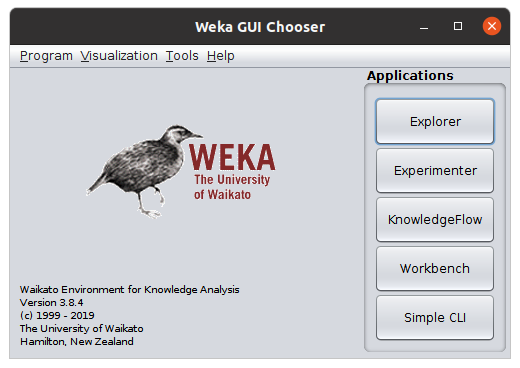
\includegraphics[width=0.4\textwidth]{imagem/weka-gui.png}
	\caption{Tela Principal do Weka}
\end{figure}

As aplicações disponíveis são:
\begin{itemize}
	\item \textbf{Explorer}: é a opção mais utilizada, com a possibilidade de trabalhar de forma interativa. È onde iremos explorar as funções da ferramenta. Focaremos principalmente nessa, pois nas outras opções realizamos muitas das funções contidas aqui, porém de forma automatizada. Esta opção permite importar dados, aplicar algoritmos de filtragem para transformar as características quantitativas em discretas ou excluir de acordo com critérios definidos.
	\item \textbf{Experimenter}: automatizar os processos, por exemplo, para rodar vários algoritmos de \textit{Machine Learning} de forma automática e visualizar todos os resultados de uma só vez.
	\item \textbf{KnowledgeFlow}: criar fluxos de processos através de uma interface com base em fluxo de dados. È possível arrastar componentes como filtros ou classificadores e conecta-los para obter novos fluxos de processamento.
	\item \textbf{Workbench}: combinar todas as outras aplicações mostradas em uma única interface. Essa pode ser interessante caso tenhamos que alternar entre as opções \textit{Explorer} e \textit{Experimenter} por várias vezes.
	\item \textbf{Simple CLI}: uma interface de linha de comando (\textit{shell}) destinada a criação de \textit{scripts shell} que podem ser utilizados com a API do Weka. Com esta API é possível rodar experimentos, algoritmos de \textit{Machine Learning} e diversas outras tarefas. Podemos automatizar tarefas e integrar aplicações.
\end{itemize}

\begin{theo}[Pasta de Trabalho do Usuário]{}
	Quando executamos o Weka pela primeira vez, no diretório raiz do usuário é criada uma pasta chamada \textbf{/wekafiles}. Nesta pasta podemos colocar os arquivos \textbf{.props} para conexão com banco de dados SQL.
\end{theo}

\section{Análise Exploratória dos Dados}
Antes de partimos para os algoritmos propriamente ditos, primeiro devemos abrir e entender um conjunto de dados. Em estatística, \textit{Exploratory Data Analysis} é uma abordagem sobre um determinado conjunto de dados para compreendermos suas características principais. Clicar em \opcbotao{Explorer}:
\begin{figure}[H]
	\centering
	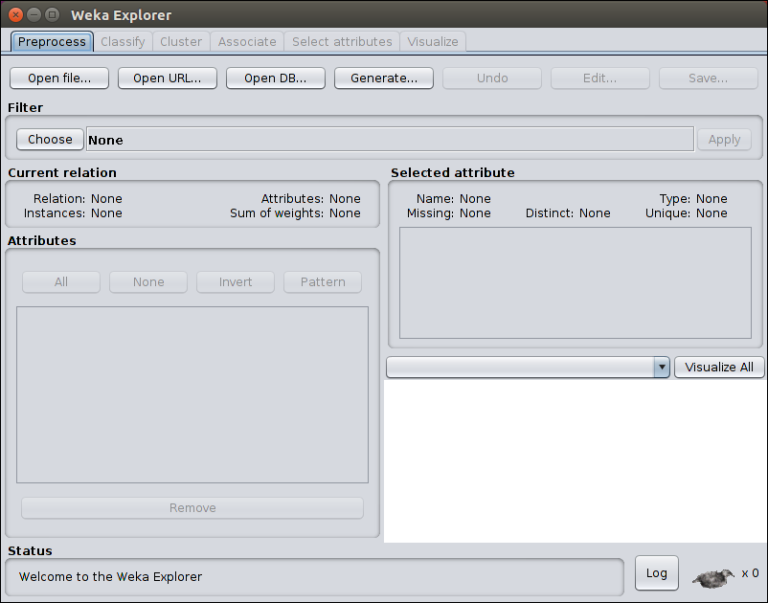
\includegraphics[width=0.5\textwidth]{imagem/weka-explorer.png}
	\caption{Opção Explorer}
\end{figure}

Abaixo das guias temos os seguintes botões para a leitura de dados: \vspace{-1em}
\begin{itemize}
	\item \opcbotao{Open file... } por padrão o Weka lê arquivos em formato ARFF (\textit{Attribute-Relation File Format}), o programa traz como exemplo algumas bases bem conhecidas.
	\item \opcbotao{Open URL... } no qual podemos obter os dados diretamente da Web.
	\item \opcbotao{Open DB... } pela disponibilização de um driver JDBC podemos ler qualquer SGBD relacional.
	\item \opcbotao{Generate... } gerar aleatoriamente uma base de dados, util para procedermos testes com os algoritmos. 
\end{itemize}
	
Como exemplo clicamos em \opcbotao{Open file... } e selecionar \textbf{WEKA\_HOME/data}:
\begin{figure}[H]
	\centering
	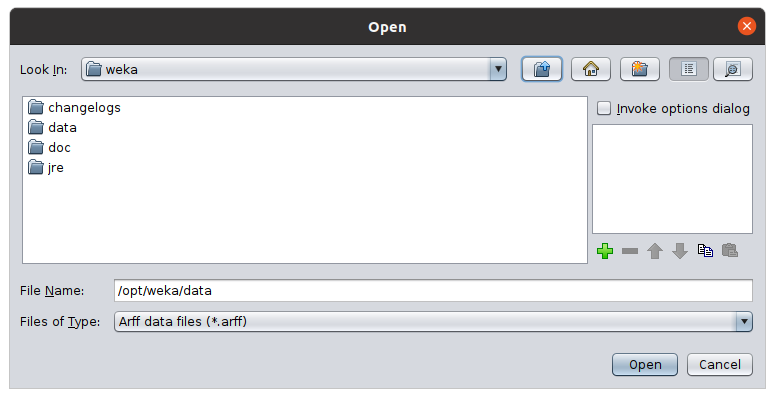
\includegraphics[width=0.4\textwidth]{imagem/diretorioData.png}
	\caption{Pastas contidas no Weka}
\end{figure}

Selecionar o dataset \textbf{iris.arff} do diretório \textbf{data} e pressionar \opcbotao{Open}:
\begin{figure}[H]
	\centering
	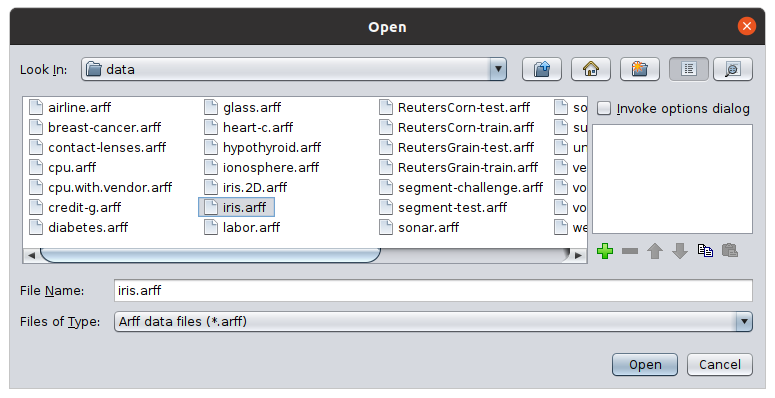
\includegraphics[width=0.4\textwidth]{imagem/arquivosARFF.png}
	\caption{Selecionar o DataSet}
\end{figure}

\begin{theo}[Não encontrou os arquivos]{}
	Não se preocupe, na página \url{https://waikato.github.io/weka-wiki/datasets/} existem vários exemplos e nesta outra \url{https://storm.cis.fordham.edu/~gweiss/data-mining/datasets.html} os mesmos arquivos ARFF disponibilizados. Criar uma pasta /data (no seu diretório de trabalho) e baixar os arquivos para esta.
\end{theo}

Após carregar o \textit{DataSet} na tela teremos uma visão geral na tela principal, são 5 atributos (colunas) e 150 instâncias (linhas). As classes ou rótulos são os tipos reais das flores. São quatro atributos preditores: \textit{SepalLength}, \textit{SepalWidth}, \textit{PetalLength}, \textit{PetalWidth} e um atributo alvo \textit{class} que identifica a espécie da Flor Iris (\textit{Setosa}, \textit{Versicolor} e \textit{Virginica}). Essa classificação foi feita por pessoas especialistas no assunto:
\begin{figure}[H]
	\centering
	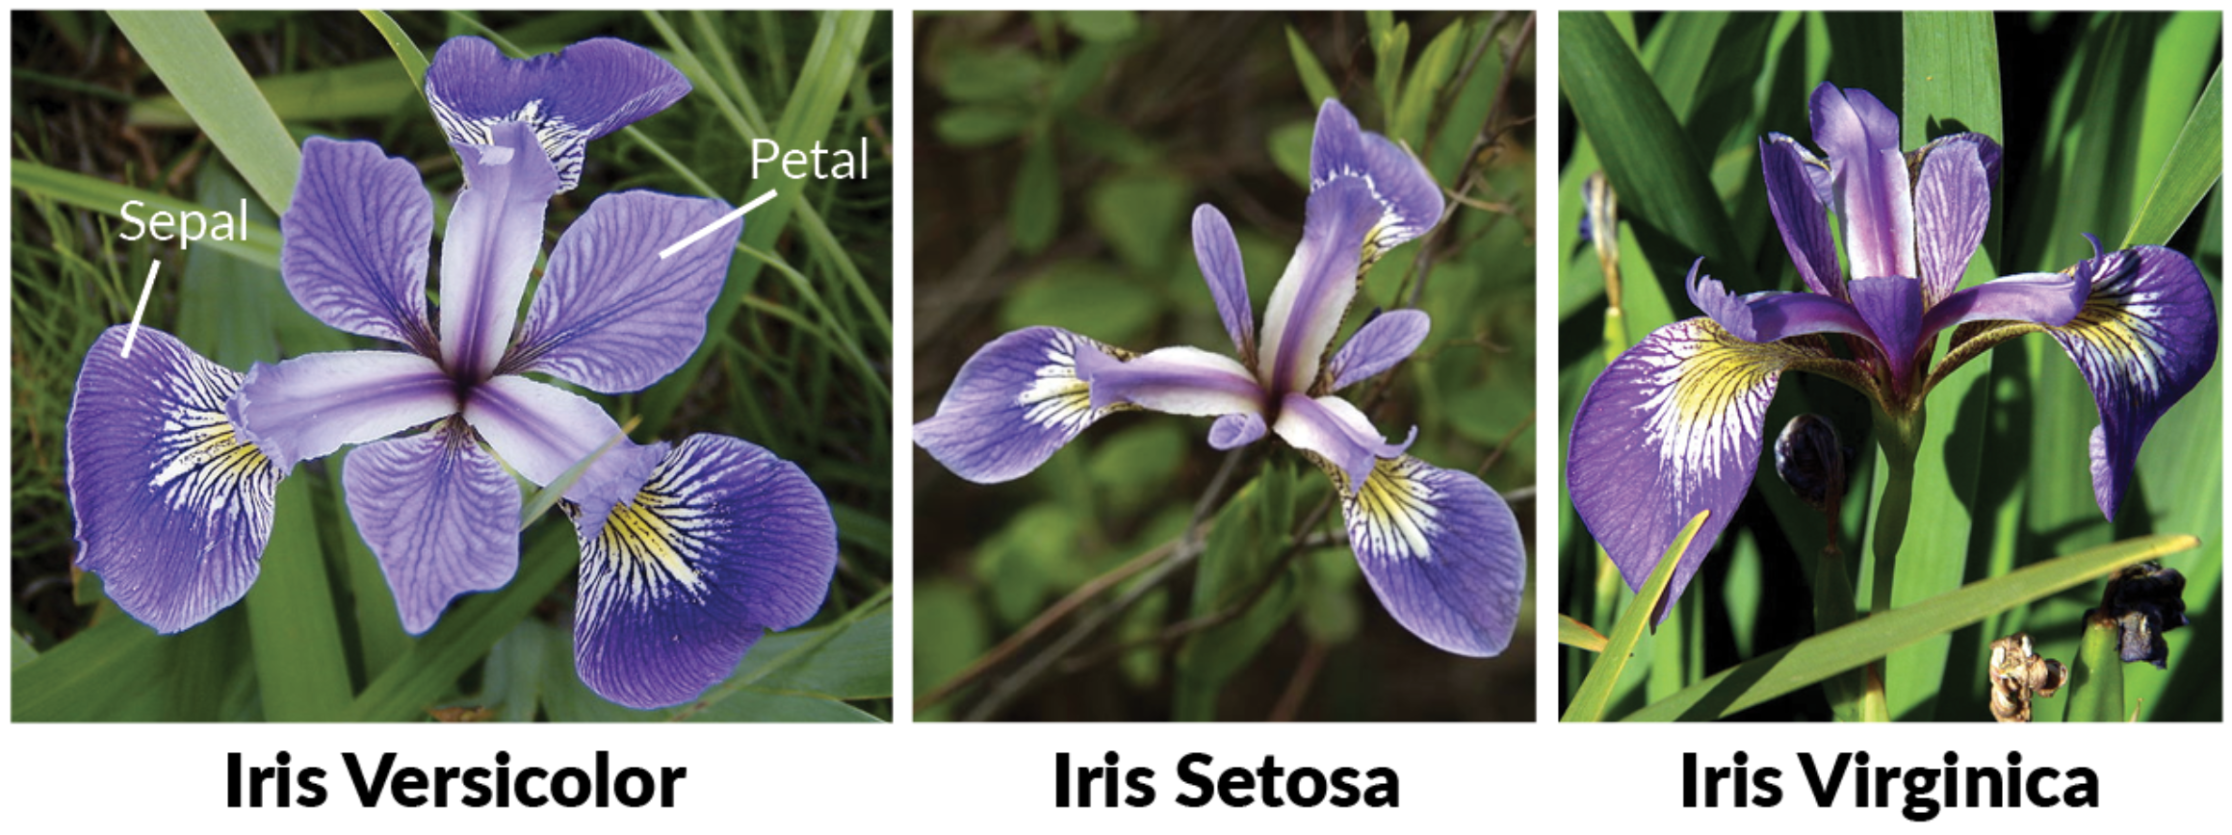
\includegraphics[width=0.65\textwidth]{imagem/iris.png}
	\caption{Tipos de Flores Iris}
\end{figure}

No botão \opcbotao{Edit... } podemos visualizar e modificar os dados. Como por exemplo, excluir uma coluna, ou modelar em um formato diferente. Neste momento vamos deixar como está. O objetivo aqui é usar esse \textit{DataSet} para aplicar os algoritmos de \textit{Machine Learning} que seja capaz de classificar corretamente a espécie de alguma flor com base nos atributos preditivos. 
\begin{figure}[H]
	\centering
	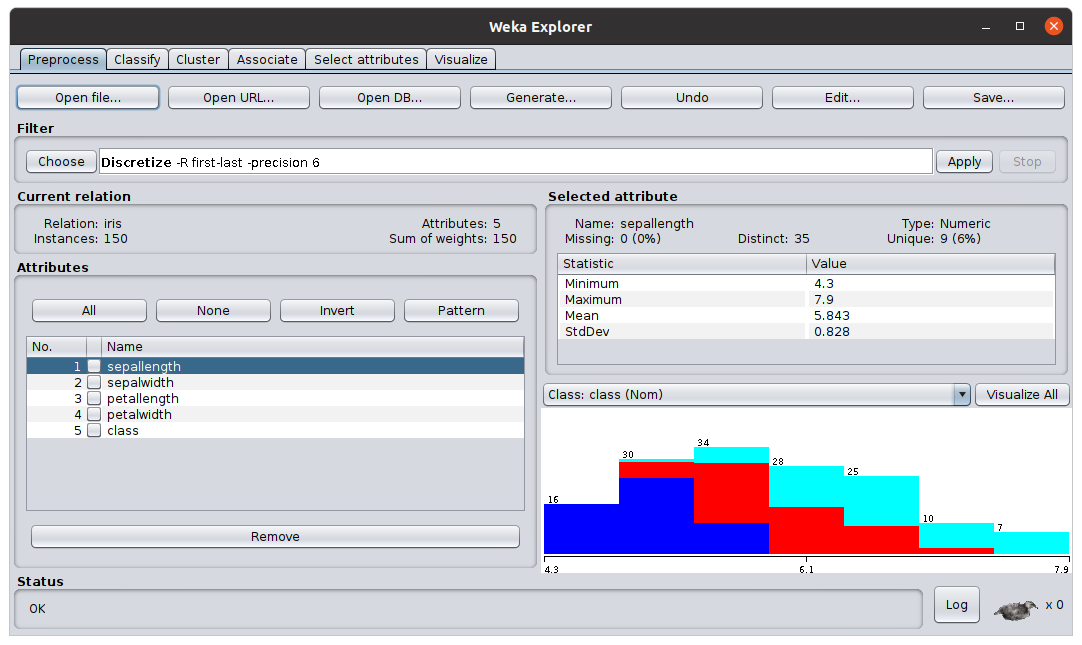
\includegraphics[width=0.6\textwidth]{imagem/explorer.png}
	\caption{Tela Principal com o DataSet Iris carregado}
\end{figure}

Essa janela é excelente para verificar os dados que temos a disposição uma vez que estão carregados, seus atributos são mostrados no box \textbf{Attributes}. Acima temos \textbf{Current Relation} que exibe o nome da relação (tabela), número de instâncias, de atributos e seus pesos. Durante a varredura dos dados, é calculado algumas estatísticas básicas para cada atributo selecionado mostradas no box \textbf{Selected attribute}. 

As ferramentas de pré-processamento no WEKA são chamadas de \textit{Filters}. São filtros para discretização, normalização, re-amostragem, transformação seleção e combinação de atributos. Algumas técnicas, como a mineração de regras de associação, só podem ser executadas em dados categóricos. Isso requer a discretização de atributos numéricos ou contínuos. Para aplicar esse filtro pressionar o botão \opcbotao{Choose } que mostra uma lista de filtros disponíveis. Selecionar \opcmenu{Supervised } $\triangleright$ \opcmenu{Attribute } $\triangleright$ \opcmenu{Discretize } e pressionar o botão \opcbotao{Apply}. O filtro converterá os valores numéricos em nominal.
\begin{figure}[H]
	\centering
	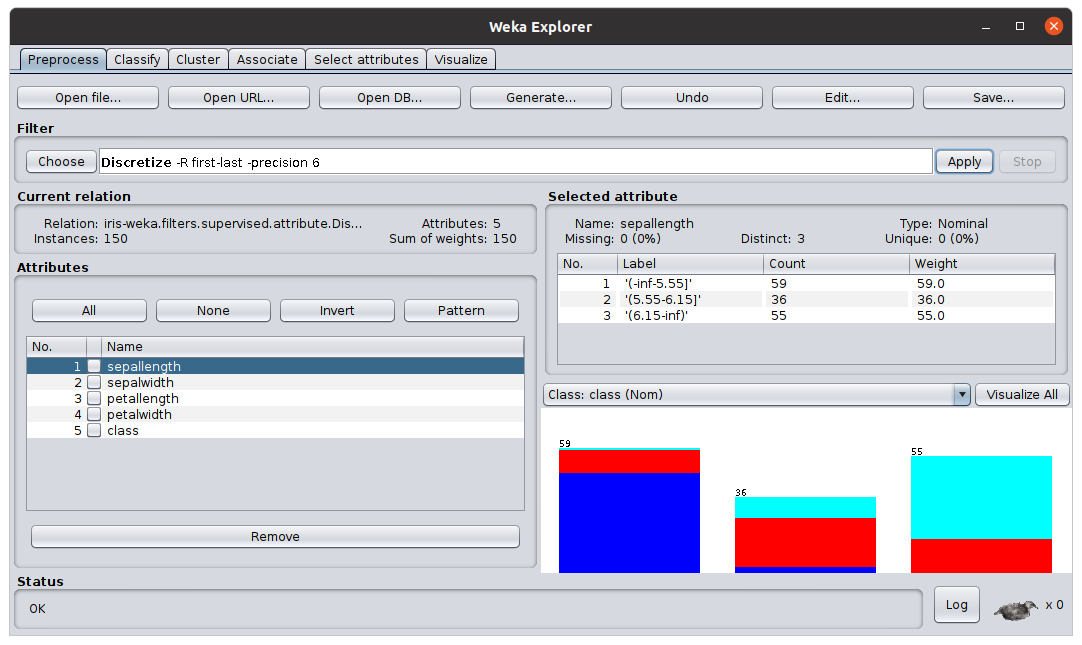
\includegraphics[width=0.6\textwidth]{imagem/filtros.png}
	\caption{Discretização Aplicada}
\end{figure}

Na parte de baixo temos uma distribuição dos dados para cada atributo selecionado ou comparação unitária quando selecionamos 2 ou mais. Podemos também visualizar todas as comparações com o botão \opcbotao{Visualize All}.

Porém a melhor maneira de visualizar esses relacionamentos e na guia superior \opcmenu{Visualize}. 
\begin{figure}[H]
	\centering
	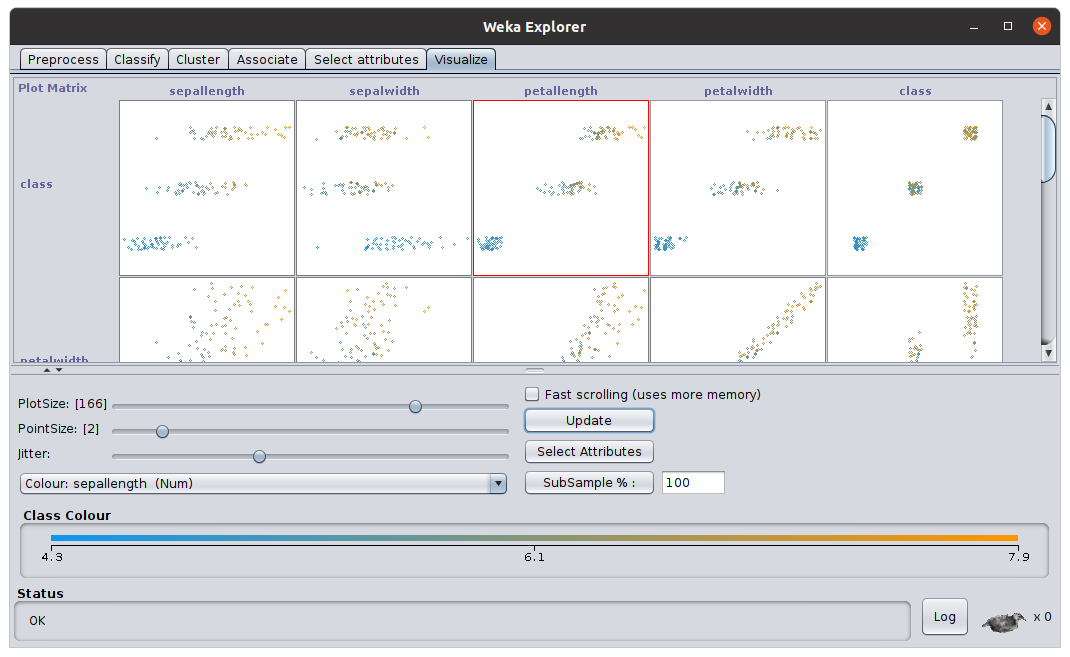
\includegraphics[width=0.6\textwidth]{imagem/visualize.png}
	\caption{Relacionamento entre os atributos}
\end{figure}

A visualização mostra um gráfico da relação entre os atributos e ajuda a determinar um problema quanto a dificuldade de aprendizagem. O botão \opcbotao{Select Attributes } é ideal para limitarmos a quantidade de atributos que desejamos visualizar e o botão \opcbotao{SubSample \% } permite definir a quantidade de dados a visualizar. 

Antes de sairmos para testar os modelos, devemos conhecer bem estas janelas para explorar melhor os dados e compreendermos o que temos a nossa disposição pois esta é uma fase extremamente importante e muitas vezes negligenciada.

\section{Executar um Algoritmo}
No Weka os algoritmos de \textit{Machine Learning} estão concentrados nas seguintes guias: \vspace{-1em}
\begin{itemize}
	\item \textbf{Classify}: os classificadores aprendem a atribuir um rótulo de classe através dos dados que foram fornecidos como exemplos. Um classificador pode reconhecer e-mails como "\textit{spam}" ou "\textit{não spam}". Temos a nossa disposição Regressão Linear e Logística, \textit{Support Vector Machines}, Árvore de Decisão, \textit{RandomForest} e \textit{Naive Bayes}.
	\item \textbf{Cluster}: a clusterização é a separação dos dados em categorias de similaridades, são disponibilizados algoritmos como: \textit{SimpleKMeans}, \textit{FilteredClusterer} e \textit{HierarchicalClusterer}.
	\item \textbf{Associate}: o aprendizado por regras de associação é um método utilizado para descobrir relações interessantes entre variáveis em grandes bancos de dados. Destina-se a identificar regras fortes descobertas em bancos de dados e se utiliza de algumas medidas de interesse. Nesta categoria temos: \textit{Apriori}, \textit{FilteredAssociator} e \textit{FPGrowth}.
\end{itemize}

O modo de executar qualquer algoritmo (Classificação, Clusterização ou Associação) é exatamente o mesmo, assim não ficaremos nesta tratando das diversas opções existentes e ao entender um único conjunto seremos capazes de realizar o mesmo processo para outros algoritmos.

Árvore de Decisão será nossa porta de entrada para esse mundo, esta é uma representação de uma tabela de decisão sob a forma de uma árvore. Para executar este com o Weka, clicar na aba \opcmenu{Classify}, pressionar \opcbotao{choose}, navegar até \opcmenu{trees } e selecionar o algoritmo \opcmenu{J48}:
\begin{figure}[H]
	\centering
	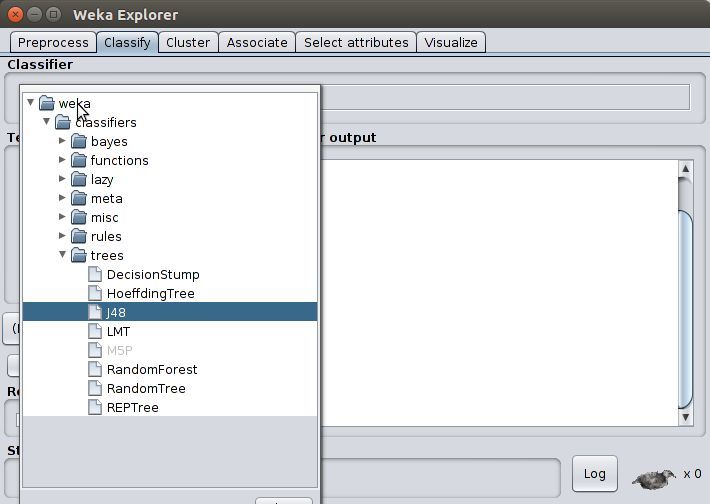
\includegraphics[width=0.45\textwidth]{imagem/weka-algoritmo-j48.png}
	\caption{Visão do J48}
\end{figure}

\textbf{J48} é uma implementação do algoritmo C4.5 na linguagem Java que utiliza uma árvore de decisão construída a partir dos dados de treino. Essas árvores são hipóteses usadas para predizer probabilidades de uma instância ser de um determinado tipo. Cada algoritmo possui uma descrição de como trabalham, para vê-la, posicionar o mouse do nome deste e uma janela amarela será aberta.

Na aba \opcmenu{Test Options } está selecionado a opção \opcmenu{Cross Validation } com \textbf{10 folds}. Isso significa que o \textit{DataSet} será treinado 9 vezes com partes distintas (\textit{folds}) dos dados. Uma parte do dado será usada como teste para classificação enquanto outras 9 partes serão usadas para treinar o modelo. Dessa forma o algoritmo é testado com todas as partes dos dados evitando erros de variância. Clicar em \opcbotao{Start } para executar o algoritmo.

As principais opções de teste disponíveis são: \vspace{-1em}
\begin{itemize}[nolistsep]
	\item \textit{Use training set}. Avalia o classificador em relação ao quão bem prediz a classe das instâncias em que foi treinado. 
	\item \textit{Supplied test set}. Permite adicionar o um conjunto de testes independente. Clicar no botão \opcbotao{Set } para adicionar o arquivo.
	\item \textit{Cross-validation}. Avalia o classificador por validação cruzada, usando o número de dobras inseridas no campo \opcbotao{Folds}. 
	\item \textit{Percentage split}. Selecionar uma certa porcentagem dos dados, que é mantida para o teste. A quantidade de dados retidos depende do valor digitado no campo \opcbotao{\%}.
\end{itemize}

Existem outras opções que podem ser acessadas através do botão \opcbotao{More options...}. Para esses dados provavelmente o resultado aparece em segundos, obviamente que se usamos uma base muito grande o tempo de espera será maior. 

Na parte inferior da janela temos a linha de status do que aconteceu. À direita temos o ícone do Weka. O número ao lado indica os vários processos que estão em execução simultaneamente. Por exemplo, ao carregar um arquivo, o pássaro se senta, isso significa que não há processos em execução (o sistema está ocioso). Ao rodar um algoritmo observe o pássaro, ele se levanta e começa a se mover, isso indica que um processo foi iniciado.

\subsection{Resultados dos Classificadores}
Após pressionarmos o botão \opcbotao{Start}, o algoritmo inicia sua tarefa, após a conclusão sua tarefa esta é marcada na \textbf{Result list} de modo que podemos alternar entre os vários relatórios armazenados. Em \textbf{Classifier output} mostra o relatório do resultado:
\begin{figure}[H]
	\centering
	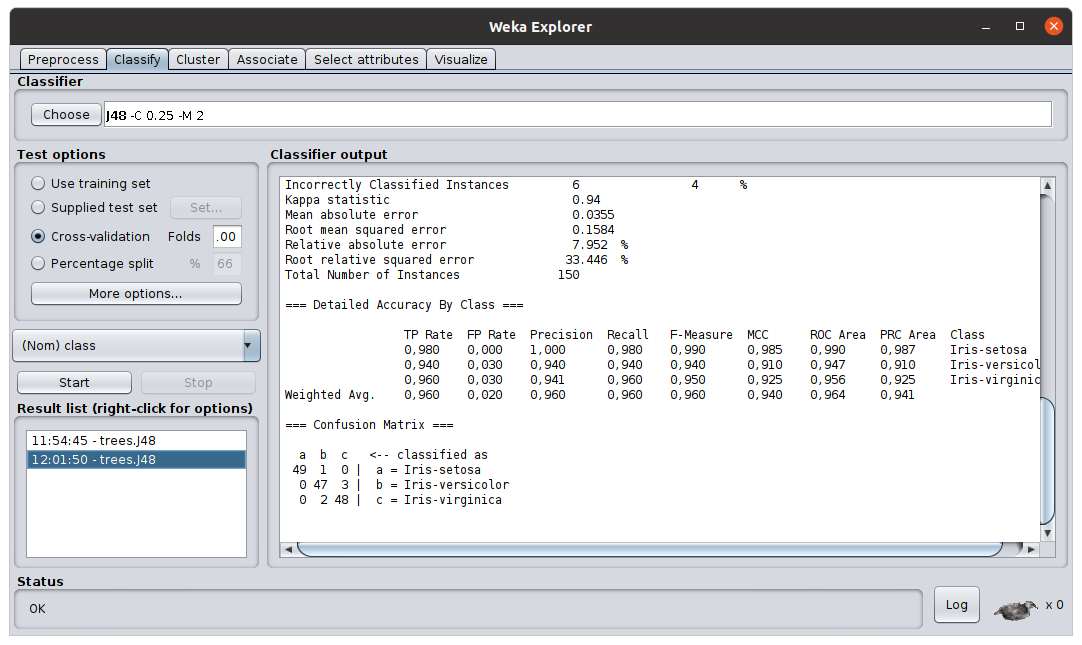
\includegraphics[width=0.7\textwidth]{imagem/resultados.png}
	\caption{Relatório de Resultados}
\end{figure}

Na seção \opcmenu{Summary}, verificamos que das 150 instâncias que foram testadas, o algoritmo acertou 144 (\textit{Correctly Classified Instances}). Isso significa que 96\% das instâncias testadas foram corretamente classificadas. Esta métrica é chamada de \textbf{Acurácia}, ou seja, nosso algoritmo teve 96\% de acertos. Na seção \opcmenu{Detailed Accuracy By Class } temos a acurácia por classe. 

Na seção \opcmenu{Confusion Matrix } é possível investigar como se saiu a classificação de cada classe comparada aos valores reais:
\begin{itemize}[nolistsep]
	\item Classe \textbf{A} (\textit{Iris-setosa}) foi classificada 1 vez como se fosse Classe \textbf{B} (\textit{Iris-versicolor}).
	\item Classe \textbf{B} foi classificada 3 vezes como se fosse classe \textbf{C} (\textit{Iris-virginica}). 
	\item Classe \textbf{C} foi classificada 2 vezes como se fosse classe \textbf{B}.
\end{itemize}
	
Essa matriz permite visualizar quais classes estão são classificadas erroneamente, ou seja, aonde o modelo está errando e precisa de mais dados para ser melhor treinado.

Escolher outros classificadores e veja o maior número de resultados possíveis, comparar os modelos, permita-se explorar bem esta tela.

\begin{theo}[Conversão de CSV para ARFF]{}
	Podemos converter facilmente um arquivo CSV para o formato nativo do Weka chamado ARFF, basta executar o seguinte comando: \\
	\codigo{java -cp weka.jar weka.core.converters.CSVLoader arq.csv > arq.arff}
\end{theo}

Weka fornece acesso direto à biblioteca de algoritmos implementados. Esse recurso possibilita a aplicação de algoritmos criados em diferentes sistemas. Por exemplo, podem ser facilmente trazidos do MATLAB e a ferramenta para acessar os algoritmos é implementada em pacotes de \textit{Machine Learning} como \textbf{Spider} e \textbf{MATLABArsenal}.

Um modelo utiliza um conjunto de dados para treinar através de cálculos a melhor maneira de mapear exemplos de dados de entrada para o resultado. Como tal, o conjunto de dados de treinamento deve ser suficientemente representativo do problema e ter muitos exemplos consistentes do atributo alvo.

\section{Gerenciador de Pacotes}
Ao retornar para a tela principal do Weka (quando iniciamos o programa) na opção \opcmenu{Tools } $\triangleright$ \opcmenu{Package Manager}, ganhamos acesso a todos os Classificadores que o Weka trabalha. Alguns desses foram criados e adicionados pela comunidade. O Gerenciador de Pacotes nos permite localizar e instalar o que desejamos trabalhar.

\begin{figure}[H]
	\centering
	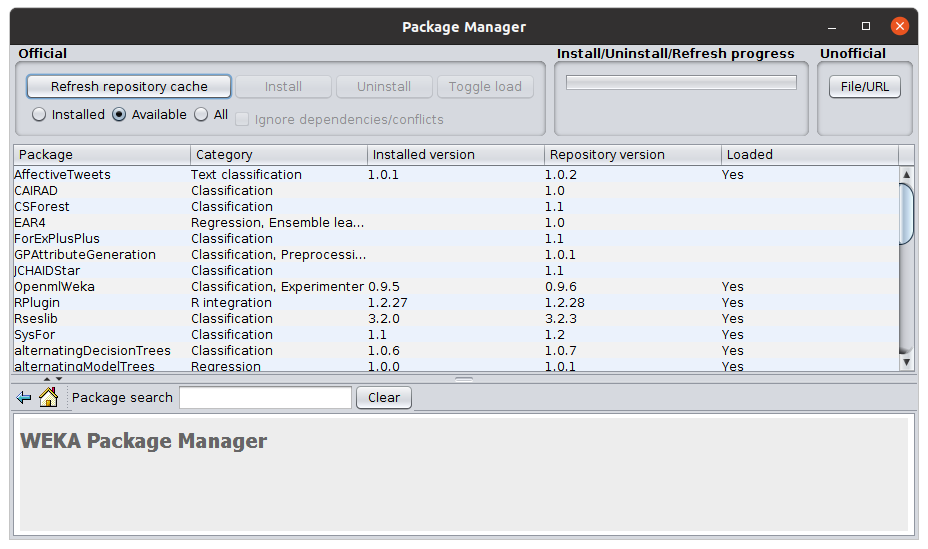
\includegraphics[width=0.45\textwidth]{imagem/packageManager.png}
	\caption{Gerenciador de Pacotes}
\end{figure}

Fornece uma lista de pacotes na parte superior da janela e um painel na parte inferior que exibe as informações sobre o pacote atualmente selecionado na lista. Podemos optar por exibir os pacotes disponíveis, apenas os instalados ou todos. A lista apresenta o nome de cada pacote, a categoria a que pertence, a versão atualmente instalada (se estiver), a versão mais recente do pacote disponível que é compatível com a versão do WEKA em uso e um campo que, para pacotes instalados, indica se o pacote foi carregado com sucesso pelo WEKA ou não.

Para atualizar qualquer pacote basta localizar um pacote aonde a coluna \textit{Installed version} seja diferente de \textit{Repository version}. Clicar neste pacote e pressionar o botão \opcbotao{Install}. 

\begin{figure}[H]
	\centering
	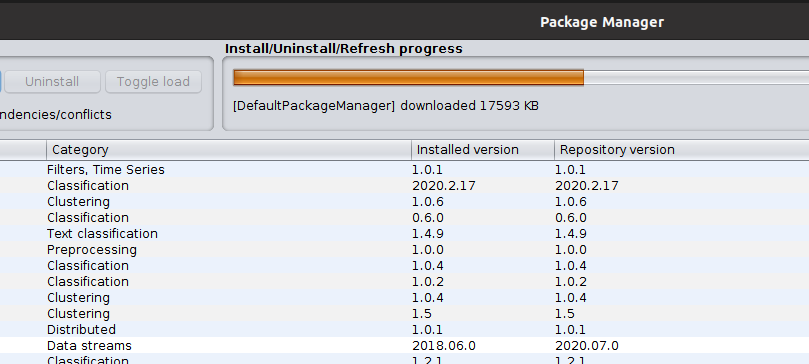
\includegraphics[width=0.45\textwidth]{imagem/installPackage.png}
	\caption{Atualizar o Pacote Data Streams}
\end{figure}

Por padrão, WEKA carrega todos os pacotes instalados, se um pacote não puder ser carregado por algum motivo, uma mensagem é exibida na coluna \textit{Loaded}. Para impedir que um pacote específico seja carregado, basta seleciona-lo e clicar no botão \opcbotao{Toggle load}. O pacote ficará marcado para a próxima vez que o WEKA for iniciado. Isso pode ser útil se um pacote instável estiver com erros, em conflito com outro (talvez devido a bibliotecas de terceiros) ou impedindo o funcionamento adequado do WEKA.
	
\section{Conectar a um banco MySQL}
Podemos consultar dados diretamente através de diversos SGBDs por um driver JDBC (\textit{Java Database Connectivity}). Isso facilita o acesso e a manipulação desses dados que estão armazenados em um banco de dados relacional como o MySQL, Oracle ou PostgreSQL.

Através de uma \textit{Query} podemos importar os dados retornados para o Weka e trabalhar normalmente com todos os filtros, métodos e classificadores sem a necessidade de gerar um arquivo de dados.

\begin{theo}[Nível Hard]{}
	O processo para obter acesso a base de dados SQL não é simples e exige que tenhamos a noção sobre como funciona a conexão JDBC e a configuração de variáveis e a URL de conexão. Nos \textit{drivers} existe a documentação do seu funcionamento, então quando for baixá-los não menosprezar sua leitura.
\end{theo}

\textbf{Passo 1}. Realizar o download do driver JDBC desejado para o SGBD e colocá-lo em uma pasta comum (por exemplo /libs).

\textbf{Passo 2}. Adicionar este arquivo (normalmente um \textbf{.jar}) a variável de ambiente CLASSPATH (no Linux isso está em um arquivo chamado /etc/environment). Por exemplo para o driver JDBC tipo 4 do SGBD MySQL: \\
\codigo{CLASSPATH=\aspas{.:/home/fernando/libs/mysql-connector-java-5.1.49.jar}}

\textbf{Passo 3}. Criar um arquivo de propriedades \textbf{DatabaseUtils.prop} que define as diversas configurações específicas sobre o SGBD que iremos nos conectar. Por exemplo, este é para o SGBD MySQL:
\begin{lstlisting}
jdbcDriver=com.mysql.jdbc.Driver
jdbcURL=jdbc:mysql://localhost:3306/conta?user=root&password=root

char=0
varchar=0
longvarchar=0
binary=0 
varbinary=0
longvarbinary=0
bit=1
numeric=2
decimal=2
tinyint=3
mallint=4
INT=5
integer=5
bigint=6
real=7
float=2
double=2
date=8
time=10
timestamp=8

CHAR=0
TEXT=0
VARCHAR=0
LONGVARCHAR=9
BINARY=0
VARBINARY=0
LONGVARBINARY=9
BIT=1
NUMERIC=2
DECIMAL=2
FLOAT=2
DOUBLE=2
TINYINT=3
SMALLINT=4 
SHORT=4
SHORT=5
INTEGER=5
BIGINT=6
LONG=6
REAL=7
DATE=8
TIME=10
TIMESTAMP=8
DATETIME=8

# Tabela de Criacao
CREATE_STRING=TEXT
CREATE_INT=INT
CREATE_DOUBLE=DOUBLE
CREATE_DATE=DATETIME
DateFormat=yyyy-MM-dd HH:mm:ss

# Opcoes do Database
checkUpperCaseNames=false
checkLowerCaseNames=false
checkForTable=true
setAutoCommit=true
createIndex=false

# Palavras reservadas
Keywords=AND, ASC, BY, DESC, FROM, GROUP, INSERT, ORDER, SELECT, UPDATE, WHERE
\end{lstlisting}

A primeira linha está o driver de conexão com o banco e a segunda a URL padrão, de resto mostra apenas como o Weka deve converter os tipos de campos do MySQL para seus tipos. Visitar esse endereço para maiores referências: \url{https://waikato.github.io/weka-wiki/weka_experiment_database_utils.props/}.

\textbf{Passo 4}. Ao entrar no Weka a partir do Menu Principal acessar a opção \opcmenu{Help } $\triangleright$ \opcmenu{SystemInfo}. 
\begin{figure}[H]
	\centering
	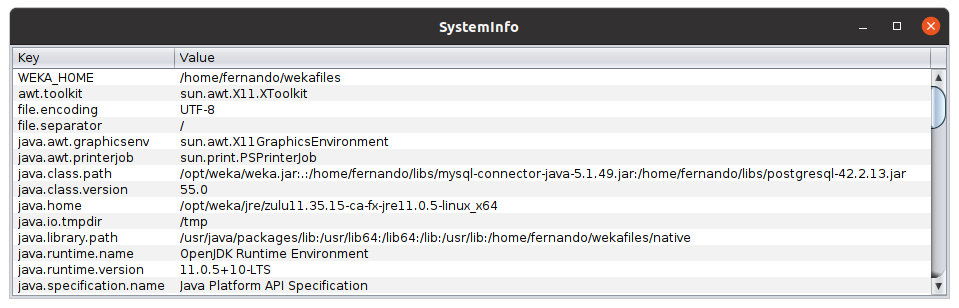
\includegraphics[width=0.7\textwidth]{imagem/systemInfo.png}
	\caption{Janela SystemInfo}
\end{figure}

Nesta janela estão contidas todas as variáveis e valores de ambientes lidos pelo programa. Observar que a variável \textbf{java.class.path} contém o arquivo jar do Driver JDBC. Caso isso não aconteça verifique se a variável \textbf{CLASSPATH} está definida corretamente, outra opção pode ser editar o arquivo \textbf{weka.sh} (ou .bat) e verificar se está inserida corretamente: \\
\codigo{CLASSPATH=\aspas{\$DIR/weka.jar:\$CLASSPATH}}

\textbf{Passo 5}. No Menu Principal acessar a opção \opcmenu{Tools } $\triangleright$ \opcmenu{SqlViewer}. 
\begin{figure}[H]
	\centering
	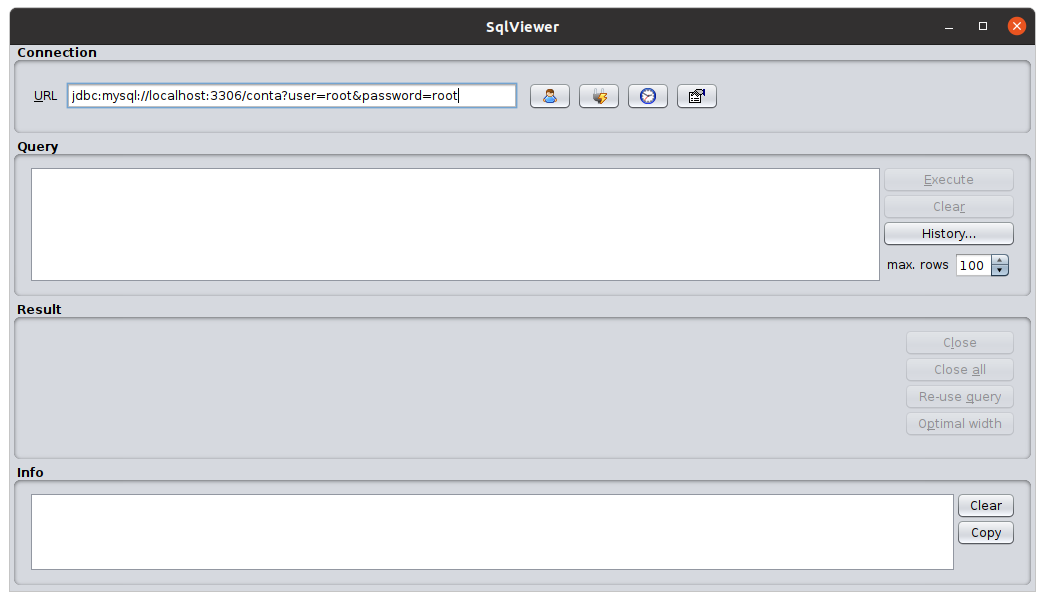
\includegraphics[width=0.6\textwidth]{imagem/SqlViewer.png}
	\caption{Janela SqlViewer}
\end{figure}

A URL que colocamos no arquivo PROPS já deve estar disponível, é possível trocá-la para acessar outra base de dados. Na frente temos uma série de botões: o primeiro permite alterar o usuário e senha (se for realizar tal ação remova essa propriedade da URL). O segundo conectar com o banco de dados. O terceiro trazer uma conexão anteriormente realizada (um histórico de conexões). O quarto ler um outro arquivo PROPS para a conexão com outro SGBD. Sendo assim podemos ter vários deles para os diferentes tipos de bases de dados.

Uma vez que tudo está sem problemas, podemos sair e entrar novamente na opção Explorer, porém ao invés de ler os dados por \opcmenu{Open File... } selecionamos a opção \opcmenu{Open DB... } e procedemos a consulta (\textit{Query}) para selecionar os dados. Ao pressionar o botão OK estes serão trazidos para que possamos proceder qualquer análise.
	
\section{Conclusão}
Weka fornece a saída estatística do processamento do modelo, também uma ferramenta de visualização para inspecionar os dados. Na realidade, existe um software que faz as mesmas coisas que os programas caros — este software se chama Weka. Através de sua interface é possível incorporar ao Weka, como qualquer outra biblioteca, a seus próprios aplicativos para fazer coisas como tarefas de mineração de dados automatizadas no lado do servidor.

Weka é um aplicativo de código aberto disponível gratuitamente sob o contrato da GNU. Originalmente escrito em C e completamente reescrito em Java, tornou-se compatível com todos os sistemas operacionais e SGBD's mais conhecidos do mercado. É amigável com uma interface gráfica que permite rápida configuração e operação principalmente para os que não possuem nenhum conhecimento de linguagem de programação. Os vários modelos podem ser aplicados ao mesmo conjunto de dados. Podemos assim comparar as saídas e selecionar o melhor que atenda ao objetivo. Isso resulta em um desenvolvimento mais rápido de modelos para \textit{Machine Learning} em geral.

Sou um entusiasta do mundo \textbf{Open Source} e novas tecnologias. Qual a diferença entre Livre e Open Source? \underline{Livre} significa que esta apostila é gratuita e pode ser compartilhada a vontade. \underline{Open Source} além de livre todos os arquivos que permitem a geração desta (chamados de arquivos fontes) devem ser disponibilizados para que qualquer pessoa possa modificar ao seu prazer, gerar novas, complementar ou fazer o que quiser. Os fontes da apostila (que foi produzida com o LaTex) está disponibilizado no GitHub \cite{github}. Veja ainda outros artigos que publico sobre tecnologia através do meu Blog Oficial \cite{fernandoanselmo}.

%--------------------------------------------------------------------------
% REFERÊNCIAS
%--------------------------------------------------------------------------
\begin{thebibliography}{4}
	\bibitem{wekaoficial} 
	Página do Weka \\
	\url{https://www.cs.waikato.ac.nz/ml/weka/}
	
		\bibitem{fernandoanselmo} 
	Fernando Anselmo - Blog Oficial de Tecnologia \\
	\url{http://www.fernandoanselmo.blogspot.com.br/}
	
	\bibitem{publicacao} 
	Encontre essa e outras publicações em \\
	\url{https://cetrex.academia.edu/FernandoAnselmo}
	
	\bibitem{github} 
	Repositório para os fontes da apostila \\
	\url{https://github.com/fernandoans/publicacoes}
\end{thebibliography}

\end{document}